\providecommand{\main}{../../../..}
\documentclass[\main/dresen_thesis.tex]{subfiles}
\begin{document}
  \begin{figure}[tb]
    \centering
    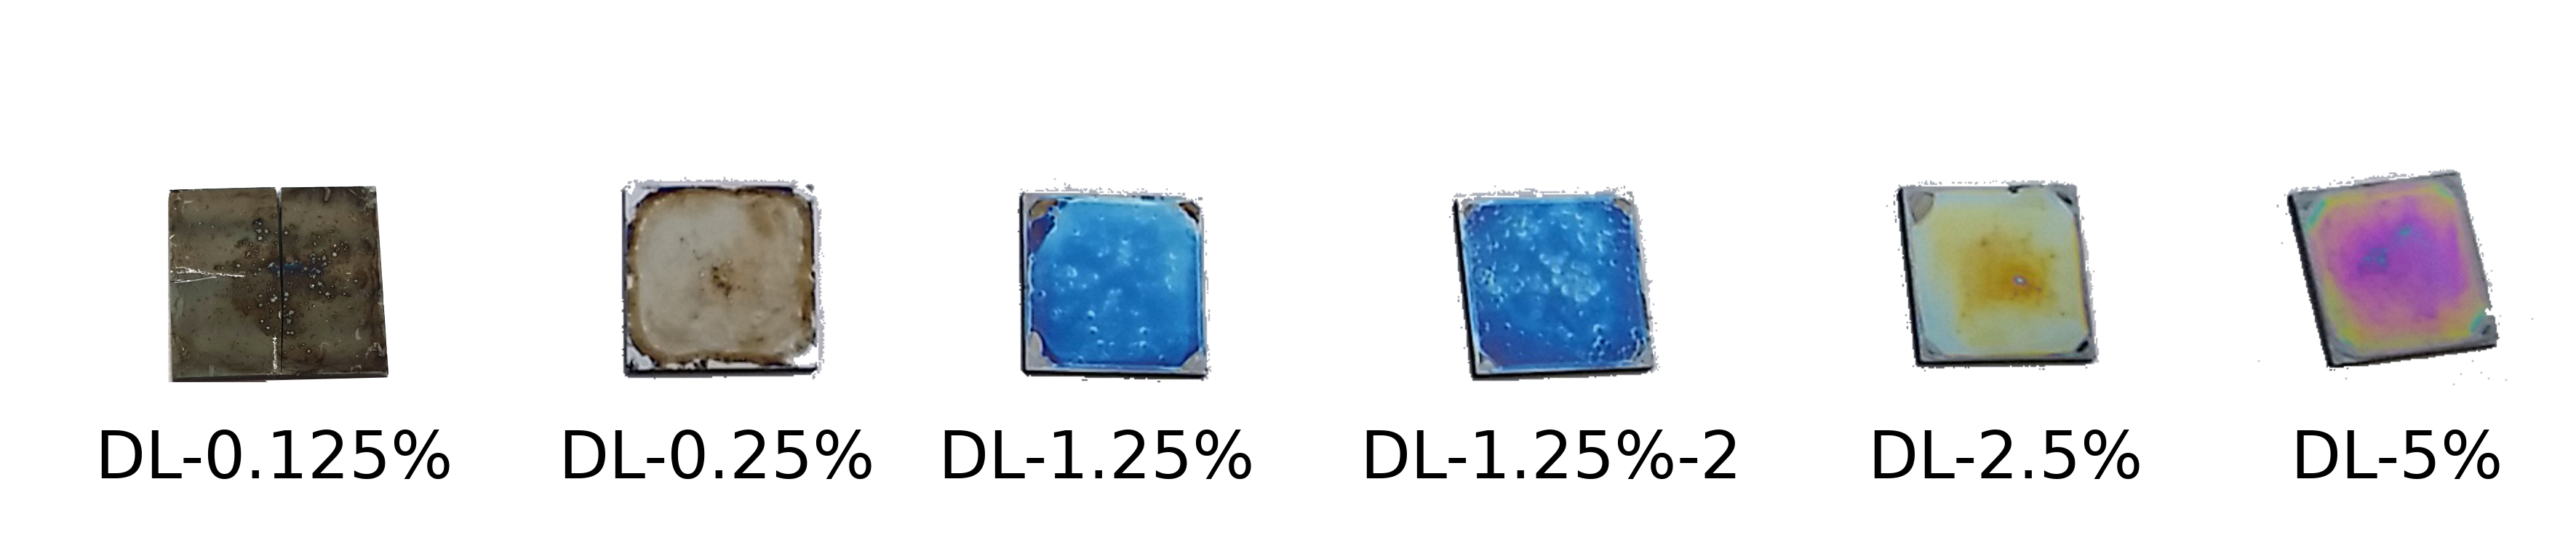
\includegraphics{doubleLayer_wafers}
    \caption{\label{fig:doubleLayers:preparation:waferImage}Image of prepared wafers}
  \end{figure}

  Describe preparation

  \begin{table}[!htbp]
    \centering
    \caption{\label{tab:doubleLayers:preparation:samples}Samples studied in this chapter.}
    \begin{tabular}{ l | l | l | l}
      \textbf{Sample}  & $c_V^\mathrm{PMMA}$ & color & characterization\\
      \hline
      DL-0.125\%    & $0.25$ & ?                & SEM, XRR, PNR\\
      DL-0.25\%     & $0.25$ & brown            & SEM(xs), XRR, PNR, VSM\\
      DL-1.25\%     & $1.25$ & blue             & SEM(xs), XRR, PNR, VSM\\
      DL-1.25-2\%   & $1.25$ & blue             & SEM, XRR\\
      DL-2.5\%      & $2.50$ & light blue/yellow& SEM(xs), XRR, PNR, VSM\\
      DL-5\%        & $5.00$ & purple           & SEM, XRR\\
      \hline
    \end{tabular}
  \end{table}

  % DL-0.50\%     & $0.50$ & brown            & SEM \\
  % DL-5\%-2      & $5.00$ & green            & SEM \\

\end{document}